
\def\Ponderation{45}
\def\SigleNumero{STT-1900}
\def\NomCours{Méthodes statistiques pour ingénieurs}
\def\DateEvaluation{24 février 2023}
\def\HeureEvaluation{18h30 à 21h20}
\def\Session{}
\def\NomEvaluation{Examen 1}

% Ne rien mettre entre les accolades si l'enseignant (ou l'enseignante) est aussi le coordonnateur (ou la coordonnatrice)
\def\Coordonnatrice{}
\def\Coordonnateur{}

% Ne rien mettre entre les accolades s'il y a plus d'une section
\def\Enseignant{Julien Miron}
\def\Enseignante{}

% Ne rien mettre entre les accolades s'il s'agit d'un cours à section unique
% Mettre le nom de chacun des enseignants et enseignantes entre les accolades
% Une case à cocher sera générée pour chacune des sections
\def\SectionA{}
\def\SectionB{} 
\def\SectionC{}
\def\SectionD{}


\def\Directives{
\begin{enumerate}
\item Matériel autorisé:
\begin{itemize}
    \item Calculatrice scientifique {\bf autorisée par la faculté des sciences et de génie};
    \item Une seule feuille aide-mémoire \textbf{manuscrite} de format lettre (8.5''$\times$11'') recto-verso.
    \end{itemize}
\item Assurez-vous que cette évaluation comporte \numquestions ~questions réparties sur \numpages{}~pages, pour un total de \numpoints{}~points.\
\item \textbf{Veuillez ne pas dégrafer votre examen.}
\item Les tables de lois se trouvent à la fin du cahier d'examen. Attention à ne rien dégrafer.
\item Ajoutez vos initiales dans le bas de chaque page (sauf pour les tables de lois).
\item Veuillez déposer votre carte d'identité \textbf{admise} avec photo sur votre bureau.\
\item Vous devez\textbf{ justifier toutes vos réponses} par une démarche claire, sauf pour les questions à choix de réponse et les vrais ou faux.\
\item Pour les questions à choix de réponse et les vrais ou faux, vous pouvez mettre un X, un crochet ($\checkmark$) ou remplir la case.
\item Le verso des feuilles peut être utilisé comme brouillon, \textbf{mais ne sera pas corrigé}. Attention à ne rien dégrafer.
\end{enumerate}
}



\documentclass{Evaluation}
\usepackage{multicol,graphicx}
\begin{document}

\newpage
%%%%%%%%%%%%%%%% QUESTION %%%%%%%%%%%%%%%%
\begin{questions}

\question[3] Laquelle des fonctions suivantes est une fonction de répartition? 

\begin{checkboxes}
\choice $F(a)=a,\ \mbox{pour } 0 <a$
		\vspace{0.3cm}
\correctchoice $ F(b) = \left\{
			\begin{array}{ll}
			0  & \mbox{ si } b<0, \\
			b & \mbox{ si } 0\leq b < 1,\\
			1 & \mbox{ si } 1 \leq b
			\end{array}
			\right. $
\choice $ F(c) = \left\{
			\begin{array}{ll}
			\sqrt{c}  & \mbox{ si } 0\leq c\leq 1, \\
			0 & \mbox{sinon}
			\end{array}
			\right. $
\choice $ F(d) = \left\{
			\begin{array}{ll}
			0  & \mbox{ si } d < -1, \\
			|d| & \mbox{ si } -1 \leq d \leq 1,\\
			1 &  \mbox{ si } 1 < d
			\end{array}
			\right. $
\end{checkboxes}



\question[3] Soit $T$, une variable aléatoire Student à 5 degrés de libertés. Nous notons $\mu_T$~et~$\sigma^2_T$, l'espérance et la variance de $T$, respectivement. Laquelle des affirmations suivantes est vraie? %module 5

\begin{checkboxes}
\choice $\displaystyle Z=\frac{T-\mu_T}{\sigma_T}\sim \mathcal{N}(0, 1)$
\choice Nous savons que $\mu_T=5$ et $\sigma^2_T=10$
\CorrectChoice La fonction de densité de $T$ est symétrique
\choice La fonction de répartition de $T$ est symétrique
\end{checkboxes}


\question[3] Laquelle des affirmations suivantes est toujours vraie au sujet de $\overline{X}=\displaystyle \frac{1}{n}\sum_{i=1}^n X_i$, où les $X_i$ sont indépendants et identiquement distribués de loi quelconque d'espérance $\mu_X$ et de variance $\sigma^2_X$? %module 5

\begin{checkboxes}
\choice $\mathbb{E}\left[\overline{X}\right]=\mu_X$ seulement si $n>30$
\vspace{0.1cm}
\correctchoice $\mathbb{E}\left[\overline{X}\right]=\mu_X$ peu importe la loi des $X_i$
\vspace{0.1cm}
\choice $\displaystyle\mathbb{E}\left[\overline{X}\right]=\mu_X$  seulement si les $X_i$ sont de loi normale
\vspace{0.1cm}
\choice $\text{Var}\left[\overline{X}\right]=\sigma^2_X$
\end{checkboxes}

\vspace{0,5cm}
\question[3] Soit $K$, $G$ et $M$ des variables aléatoires indépendantes qui suivent respectivement une khi-carré à 4 degrés de liberté, une Student à 3 degrés de liberté et une Fisher à 3 et 4 degrés de liberté. 

Que vaut $P(K>1,06~\cap~G~>~0,277~\cap~M~<~16,69)$?

\begin{oneparcheckboxes}
		\correctchoice 0,3564
		\choice 0,5346
		\choice 0,0036
		\choice 0,0054
		\choice 0,0396
\end{oneparcheckboxes}

\vspace{0,5cm}
\question[3]\label{normaleBivariee}
Soit un système électronique constitué d'un composant de type 1 et d'un composant de type 2. Considérons ${X}_1 $ et ${X}_2 $, deux variables aléatoires qui représentent respectivement la durée de vie (en mois) du composant de type 1 et celle du composant de type 2. On suppose que la loi conjointe de (${X}_1 $ , ${X}_2 $) est une loi normale bidimensionnelle de paramètres ${\mu}_1 $ = 92, ${\mu}_2 $ =84, ${\sigma}_1 ^2$= 9 , ${\sigma}_2 ^2$=  25 et $\rho $=0,8.

Sachant que la durée de vie du composant de type 1 vaut 101 mois, identifiez la loi de la durée de vie du composant de type 2.

 \begin{oneparcheckboxes}
		\choice $\mathcal{N}(92, \; 9)$  %  X1
		\correctchoice $\mathcal{N}(96,\;9)$ % X_2 | X1
		\choice $\mathcal{N}(84,\; 25)$ % X_2 
		\choice $\mathcal{N}(100, \; 9)$ % X_1 | X2
		\choice $\mathcal{N}(144, \; 9)$ % X_2 | X1 avec sigma^2 plutot que sigma
\end{oneparcheckboxes}

\begin{solution}
On cherche la loi de
		\begin{eqnarray*}
			{X}_2|{X}_1=101 &\sim& N\left(\mu_2 +\rho\, \sigma_2\, \left(\frac{x_1-\mu_1}{\sigma_1}\right),\sigma_2^2 \,\left(1-\rho_2^2\right)\right)\\
			&\sim& N\left(84 +0.8\times 5\times \left(\frac{101-92}{3}\right),25 \,\left(1-0.8^2\right)\right)\\
			&\sim& N\left(96, 9 \right)
	\end{eqnarray*}
\end{solution}


\newpage


\newpage
\question\label{pa} On définit les événements $A$, $B$ et $C$ et les probabilités $P(A)$, $P(B)$ et $P(C)$. Que vaut $P(A)$ dans les cas suivants?
\begin{parts}
    \part[3] $A$ et $B$ sont indépendants, $P(B)=0,3$ et $P(A\cup B)= 0,7$?
\begin{solution}
Solution:
\begin{align*}
    P(A\cap B)=&P(A)+P(B)-P(A\cup B)\\
    P(A)P(B)=&P(A)+P(B)-P(A\cup B) \text{ car } A\perp B\\
    0,3 P(A)= & P(A)+0,3-0,7\\
    0,7P(A)=& 0,4\\
    P(A)=&4/7
\end{align*}
\end{solution}

\vspace{7cm}
\part[3] $A\subset B$, $P(A\cup B)=0,5$ et $P(A\cap B)=0,1$?
\begin{solution}
Solution:
Comme $A \subset B$, on sait que $P(A)=P(A\cap B)$, donc $P(A)=0,2$.
\end{solution}

\vspace{7cm}
\part[3] $B\subset A$, $P(A\cup B)=0,5$ et $P(A\cap B)=0,1$?
\begin{solution}
Solution:
Comme $B \subset A$, on sait que $P(A)=P(A\cup B)$, donc $P(A)=0,4$.
\end{solution}
\vspace{7,5cm}
\pagesuivante{\ref{pa}}
\newpage
\suite{\ref{pa}}
\part[3] $P(A|B)=0,3$, $P(A\cup B)=0,4$ et $P(B)=0,2$?
\begin{solution}
Solution:
\begin{align*}
    P(A| B)=&\frac{P(A\cap B)}{P(B)}\\
    P(A| B)=&\frac{P(A)+P(B)-P(A\cup B)}{P(B)}\\
    0,3=&\frac{P(A)+0,2-0,4}{0,2}\\
    P(A)=&0,8
\end{align*}
\end{solution}

\vspace{9cm}
\part[3] $B$ et $C$ forment une partition de l'espace échantillonnal, et $P(A\cap C) = 0,1$, $P(C)=0,6$ et $P(A|B)~=~0,25$.
\begin{solution}
\begin{align*}
    P(A)=&P(A \cap B) + P(A\cap C)\\
\end{align*}
On cherche $P(A\cap B)$. 

\begin{align*}
    P(A\cap B)=&P(B)P(A|B)\\
    P(A\cap B)=&0,4\cdot 0,25\\
    P(A\cap B)=&0,1\\
\end{align*}
Donc $P(A)=0,1+0,1=0,2$
\end{solution}

\end{parts}

\newpage
\question[10]
Déterminez si les énoncés suivants sont vrais ou faux. 

\textbf{\textit{Une bonne réponse vaut 2 points, une mauvaise réponse vaut -1 point et une réponse vide vaut 0 point, pour un total minimum de 0 point.}}

\begin{parts}
    \part Si $X_1,\hdots,X_{25}$ constituent un échantillon aléatoire simple issu d'une distribution $\mathcal{N}(0; 1)$, alors la moyenne échantillonnale de ces 25 valeurs suit une loi $\mathcal{N}(0; 1)$. 

    \begin{oneparcheckboxes}
        \choice Vrai
        \correctchoice Faux
    \end{oneparcheckboxes}

    \begin{solution}
        Faux
    \end{solution}
    \vspace{0.5cm}
    \part Si $X_1,\hdots,X_{17}$ constituent un échantillon aléatoire simple issu d'une distribution $\mathcal{N}(5; 4)$, alors la variable $16S^2$ a une espérance de 16 et une variance de 32. 

    \begin{oneparcheckboxes}
        \correctchoice Vrai
        \choice Faux
    \end{oneparcheckboxes}
        \begin{solution}
        Vrai
    \end{solution}
        \vspace{0.5cm}

    \part Si $W$ suit une $\chi^2_4$ (khi-carré avec $4$ degrés de liberté), alors la densité de $W$ est symétrique. 

    \begin{oneparcheckboxes}
        \choice Vrai
        \correctchoice Faux
    \end{oneparcheckboxes}
    
    \begin{solution}
        Faux
    \end{solution}
        \vspace{0.5cm}
    \item Le poids des tomates d'un certain agriculteur suit une loi normale de moyenne $300\text{ grammes}$ et de variance $100\text{ grammes}^2$. On prend des mesures sur 25 tomates choisies aléatoirement et on obtient une moyenne échantillonnale de $309,12\text{ grammes}$ et une variance échantillonnale de $118,3\text{ grammes}^2$. Dans cette situation, les nombres $309,12$ et $118,3$ sont des paramètres et les nombres $300$ et $100$ sont des statistiques.
    
    \begin{oneparcheckboxes}
        \correctchoice Vrai
        \choice Faux
    \end{oneparcheckboxes}
            \begin{solution}
        Vrai
    \end{solution}
        \vspace{0.5cm}

    \part Si $T\sim t_{3}$ (Student avec 3 degrés de liberté), alors $P(T>3)=P(T<3)=0,50$. 

    \begin{oneparcheckboxes}
        \choice Vrai
        \correctchoice Faux
    \end{oneparcheckboxes}
    
        \begin{solution}
        Faux
    \end{solution}
        \vspace{0.5cm}

    \part Soit deux échantillons aléatoires indépendants de taille $n_1=26$ et $n_2=26$ qui proviennent de lois normales $\mathcal{N}(\mu_1, \sigma^2)$ et $\mathcal{N}(\mu_2, \sigma^2)$. Les moyennes échantillonnales sont respectivement $\overline{X}_1$ et $\overline{X}_2$, alors que les variances échantillonnales sont respectivement $S^2_1$ et $S^2_2$. La statistique $S^2_1/S^2_2$ suit une $F_{25,25}$. 

    \begin{oneparcheckboxes}
        \correctchoice Vrai
        \choice Faux
    \end{oneparcheckboxes}
    
            \begin{solution}
        Vrai
    \end{solution}

    \end{parts}
\newpage
\question \label{introproba} Soit les trois expériences aléatoires suivantes:
\begin{itemize}
    \item $\mathcal{E}_1$: On lance un dé équilibré à 6 faces et on note la face du dessus;
    \item $\mathcal{E}_2$: On lance une balle de baseball et on mesure la distance parcourue en mètres;
    \item $\mathcal{E}_3$: On frappe une balle de golf et on mesure la distance parcourue en mètres.
\end{itemize}

On note les variables aléatoires suivantes:
\begin{itemize}
    \item $D$: le chiffre de la face du dessus du dé;
    \item $B$: la distance parcourue par une balle de baseball, en mètres, jusqu'à son arrêt complet;
    \item $G$: la distance parcourue par une balle de golf, en mètres, jusqu'à son arrêt complet.
\end{itemize}

\begin{parts}
\part[2] Quels sont les espaces échantillonnaux $S_1$ et $S_2$ des expériences $\mathcal{E}_1$ et $\mathcal{E}_2$ respectivement?
\begin{solution}
Solution: 
$S_1=\{1,2,3,4,5,6\}$ et $S_2=\mathbb{R}^+$ ou $S_2=[0, +\infty[$
\end{solution}
\vspace{6cm}
\part[3] Nous savons que la balle de golf a été frappée plus loin que 150 mètres. Sachant cela, nous nous intéressons à la probabilité que la balle ait parcouru au moins 175 mètres. Comment calculerions-nous cette probabilité? Votre réponse doit être la plus simplifiée possible. \textit{Ici, on cherche une expression mathématique de cette probabilité, pas une réponse précise.}
\begin{solution}
Solution: 

On cherche la probabilité que la balle parcourt plus de 35 \textbf{sachant} qu'elle a parcouru plus de 30: 

$\mathbb{P}(B>35 | B>30)=\displaystyle \frac{\mathbb{P}(B>35 \cap B>30)}{\mathbb{P}(B>30)}=\frac{\mathbb{P}(B>35)}{\mathbb{P}(B>30)}$
\end{solution}

\vspace{10cm}
\pagesuivante{\ref{introproba}}
\newpage
\suite{\ref{introproba}}

\part[6] Nous apprenons maintenant que la variable aléatoire $B$ suit une loi normale d'espérance $30$ mètres et de variance~$9$ mètres$^2$, et que chaque lancer est indépendant des autres. Si quatre balles de baseball sont lancées, quelle est la probabilité que la somme des distances parcourues par les quatre balles soit plus grande que 126 mètres?
\begin{solution}
Solution: 
Comme $B$ suit une normale, $B_1+B_2\sim \mathcal{N}(30+30= 60, 8 +8 =16)$. On cherche $\mathbb{P}(B_1+B_2 >64)$:

$\mathbb{P}(B_1+B_2 >64)=\mathbb{P}\left(\displaystyle \frac{(B_1+B_2)-60}{4} >\frac{64-60}{4}\right)= \mathbb{P}(Z > 1)$, où $Z\sim \mathcal{N}(0,1)$

$\mathbb{P}(Z > 1)=1-\Phi(1)\approx 1- 0,84134= 0,15866$
\end{solution}

\vspace{10cm}
\part[6] La variable aléatoire $G$ n'est pas symétrique, mais son espérance est $300$~mètres, sa variance est $810$~mètres$^2$ et chaque balle frappée est indépendante des autres. Si 90 balles de golf sont frappées, quelle est la probabilité que la moyenne des distances parcourues par ces 90 balles soit inférieure à 294 mètres?
\begin{solution}
Solution: 
$G$ suit une loi \textit{quelconque}, mais comme $n\geq 30$, on utilise le TCL.

On sait que $\bar{G}=\displaystyle \frac{G_1+\hdots+G_{90}}{90}\approx \mathcal{N}\left(200, \frac{810}{90}\right)$.

On a donc $\mathbb{P}(\bar{G}<194)=\mathbb{P}\left(\displaystyle \frac{\bar{G}-200}{3} < \frac{194-200}{3}\right)\approx \mathbb{P}\left(\displaystyle Z < -2\right)$, où $Z\sim\mathcal{N}(0,1)$

$\mathbb{P}\left(\displaystyle Z < -2\right)=1-\Phi(2)=0,02275$
\end{solution}
\newpage
\end{parts}

\question \label{CDF} La variable aléatoire $X$ a la fonction de répartition continue suivante:
\begin{center}
    $F(x)=\left\{
			\displaystyle \begin{array}{ll}
   			0 & \mbox{ si } x < 0,\\
			\displaystyle \frac{\sqrt{x}}{5}  & \mbox{ si } 0\leq x \leq u, \\
                1 & \mbox{ si } u < x.

			\end{array}
			\right.$
\end{center}
\begin{parts}
\part[3] Que vaut $u$?
\begin{solution}
Solution: 
Nous voulons que $F(a)-F(0)=1$, donc $\displaystyle \frac{a^3}{8}=1$, ainsi $a=2$.
\end{solution}

\vspace{7cm}
\part[3] Quelle est la fonction de densité de $X$? \textit{Si vous n'avez pas trouvé «$u$» à la question précédente, vous pouvez exprimer la densité avec «$u$».}
\begin{solution}
Solution: 
Nous savons que $f(x) = \displaystyle \frac{d}{dx}F(x)$, d'où

\begin{center}
    $f(x)=\left\{
			\displaystyle \begin{array}{ll}
   			0 & \mbox{ si } x < 0,\\
			\displaystyle \frac{3x}{8}  & \mbox{ si } 0\leq x \leq 2, \\
                0 & \mbox{ si } x > 2.

			\end{array}
			\right.$
\end{center}

\end{solution}
\vspace{12cm}

\pagesuivante{\ref{CDF}}
\newpage
\suite{\ref{CDF}}
\part[4] Quelle est la probabilité que $X$ soit supérieur à $9$, sachant que $X$ est entre $4$ et $16$?
\begin{solution}
Solution: 
\begin{align*}
    P(X>1|0,5<X<1,5) = &\displaystyle \frac{P(X> 1 \cap 0,5<X<1,5)}{P(0,5>X>1,5)}\\
    =& \frac{P(1<X<1,5)}{P(0,5<X<1,5)}\\
    =&\frac{F(1,5)-F(1)}{F(1,5)-F(0,5)}\\
    =&\frac{1,5^3-1}{1,5^3-0,5^3}\\
    =&\frac{2,375}{3.250}\approx 0,731
\end{align*}

\end{solution}

\vspace{10cm}
\part[3] Soit les quantités suivantes:

\begin{align*}
    \int_{-\infty}^{+\infty}xf(x)dx = \frac{25}{3}, & & \int_{-\infty}^{+\infty}x^2f(x)dx = 125,
\end{align*}
où $f(x)$ est la fonction de densité de $X$.

Quel est l'écart-type de $X$?
\end{parts}
\begin{solution}
Solution: 
On utilise $\text{Var}(X)=E(X^2)-E(X)^2=2,4-1,5^2=0,15$.

L'écart-type est la racine de la variance donc $\sigma = \sqrt{0,15}\approx0,387$
\end{solution}
\newpage


  \question \label{conjointe} Soit $X$ et $Y$ deux variables aléatoires dont la loi conjointe est 
$$f(x,y)=\left\{
			\begin{array}{ll}
   \displaystyle \frac{1}{(\alpha-1) (\beta-10)}  & \mbox{ si } 1\leq x\leq \alpha , \ \ 10\leq y\leq \beta \\
    0  & \mbox{ sinon. }
			\end{array}
			\right.$$

Les variables $X$ et $Y$ sont indépendantes et
    $$f_X(x)=\left\{
			\begin{array}{ll}
		\displaystyle	\frac{1}{\alpha-1}  & \mbox{ si } 1\leq x \leq \alpha\\
			0  & \mbox{ sinon. } 
			\end{array}
			\right.$$

Dans ces fonctions de densité, $\alpha > 1$ et $\beta>10$.
\begin{parts}
\part[6] Quelle est la loi marginale de $Y$?

\begin{solution}
Première méthode. Comme $X$ et $Y$ sont indépendants, $f(x,y)=f_X(x)f_Y(y)$. Donc 

$$\frac{\lambda^2\exp(-\lambda x) \alpha y^{\alpha-1}}{(1+\lambda y^{\alpha})^2} = \lambda\exp(-\lambda x) f_Y(y)$$

d'où 


    $$f_Y(y)=\left\{
			\begin{array}{ll}
		\displaystyle	\frac{\lambda \alpha y^{\alpha-1}}{(1+\lambda y^{\alpha})^2}  & \mbox{ si } 0\leq y \\
			0  & \mbox{ sinon. } 
			\end{array}
			\right.$$

Deuxième méthode. On intègre par rapport à $x$.

\begin{align*}
    f_Y(y)=&\frac{\lambda^2 \alpha y^{\alpha-1}}{(1+\lambday^\alpha)^2}\int_0^{\infty} \exp(-\lambda x) dx\\
        =& \frac{\lambda^2 \alpha y^{\alpha-1}}{(1+\lambday^\alpha)^2} \left. \frac{-\exp(-\lambda x)}{\lambda}\right|_{x=0}^{\infty}\\
        =& \frac{\lambda \alpha y^{\alpha-1}}{(1+\lambday^\alpha)^2}(0--1)
\end{align*}
   $$f_Y(y)=\left\{
			\begin{array}{ll}
		\displaystyle	\frac{\lambda \alpha y^{\alpha-1}}{(1+\lambda y^{\alpha})^2}  & \mbox{ si } 0\leq y \\
			0  & \mbox{ sinon. } 
			\end{array}
			\right.$$
\end{solution}

\vspace{18cm}

\pagesuivante{\ref{conjointe}}
\newpage
\suite{\ref{conjointe}}
\part[6] Si $\alpha =8$, calculez $P(1\leq X\leq 6)$.


\begin{solution}
\begin{align*}
    P(0\leq X\leq 1) =& \int_{0}^1 f_X(x)dx\\
    =& \int_{0}^1 \frac{1}{2}\exp(-\frac{x}{2})dx\\
    =& \left. -\exp(-\frac{x}{2})\right|_0^1\\
    =& 1-\exp(-1/2)\\
    \approx& 0,3935
    \end{align*}
\end{solution}


\end{parts}
\newpage
\question[]\label{micro}
Dans un laboratoire de microtechnique, un technicien a étudié le temps de réaction (en millisecondes) d'un certain type de détecteur de mouvements. Les 21 valeurs suivantes sont des temps de réaction collectés au cours d'une journée:

\begin{center}
\begin{tabular}{  c c c c c c c c }
111  &111  &111  &112  &113  &113  &113 \\
113 &115  &115  &115  &115 &115 & 116 \\
116 & 118 & 118 & 119 & 125 &127 & 128\\
\end{tabular}
\end{center}

Le diagramme en boîte ci-dessous a été tracé à partir de ces résultats. Il manque toutefois quelque chose à ce diagramme (il ne s'agit pas d'un titre ou de noms d'axes).

\medskip

\begin{parts}
\part[3] Ajoutez \textbf{sur le diagramme} l'élément manquant et dites ce que vous avez fait (ceci \textit{doit} inclure des calculs) sous le diagramme.
\begin{center}
		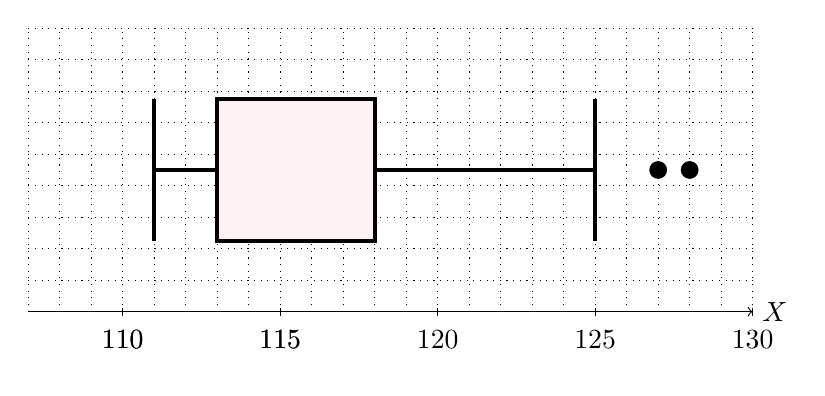
\begin{tikzpicture}[x=0.4cm,y=0.9cm]
         \draw[step=0.4cm,,dotted,color=black] (107,0) grid (130,4);
		\draw[->] (107,0) -- (130,0) node[right] {$X$} ;
		\foreach \X in {110,115,110,115,120,125,130} {
			\draw (\X,0.05cm) -- (\X,-0.05cm) node[below] {$\X\strut$};}
		\draw[ultra thick][fill=red!5] (113,1) rectangle (118,3);
		\draw[ultra thick] (111,1) -- (111,3);
		\draw[ultra thick] (111,2) -- (113,2);
		\draw[ultra thick] (118,2) -- (125,2);
		%\draw[ultra thick] (4,1) -- (4,3);
		\draw[ultra thick] (125,1) -- (125,3);
        \filldraw [black] (127, 2) circle (3pt);
        \filldraw [black] (128, 2) circle (3pt);
			\end{tikzpicture}\\
	\end{center}
 \begin{solution}
     Il manque la médiane à (114 + 114) /2 = 114
 \end{solution}
\vspace{13cm}

\pagesuivante{\ref{micro}}
\newpage
\suite{\ref{micro}}

\part[6] Nous apprenons que la plus grande observation (128) est erronée. Nous ne connaissons pas sa valeur, mais nous savons que celle-ci est plus grande que 150. Nous notons cette valeur XXX et nous savons que XXX~$>$~150. Le nouveau jeu de données est donc:

\begin{center}
\begin{tabular}{  c c c c c c c c }
111  &111  &111  &112  &113  &113  &113 \\
113 &115  &115  &115  &115 &115 & 116 \\
116 & 118 & 118 & 119 & 125 &127 & XXX\\
\end{tabular}
\end{center}

À partir de ce nouveau jeu de données, répondez aux questions suivantes. Nous nommons «jeu de données original» celui qui contient l'observation 128 et «nouveau jeu de données» celui qui contient l'observation XXX.

Déterminez si les énoncés suivants sont vrais ou faux. 

\textbf{\textit{Une bonne réponse vaut 2 points, une mauvaise réponse vaut -1 point et une réponse vide vaut 0 point, pour un total minimum de 0 point.}}

\begin{subparts}
\subpart La médiane échantillonnale du nouveau jeu de données est supérieure à celle du jeu de données original.

    \begin{oneparcheckboxes}
        \choice Vrai
        \correctchoice Faux
    \end{oneparcheckboxes}
    
\begin{solution}
    Faux
\end{solution}

\subpart La moyenne échantillonnale du nouveau jeu de données est supérieure à celle du jeu de données original.

    \begin{oneparcheckboxes}
        \correctchoice Vrai
        \choice Faux
    \end{oneparcheckboxes}
    
\begin{solution}
    Vrai
\end{solution}

\subpart La variance échantillonnale du nouveau jeu de données est supérieure à celle du jeu de données original.

    \begin{oneparcheckboxes}
        \correctchoice Vrai
        \choice Faux
    \end{oneparcheckboxes}
    
\begin{solution}
    Vrai
\end{solution}

\end{subparts}
\end{parts}

\newpage
\question\label{estimateursPonctuels} 

Soit $X_1, \hdots, X_9$ un échantillon aléatoire d'une variable $X\sim\mathcal{N}(12, 4)$. Nous avons que $X_1, \dots, X_9$ sont indépendantes. 

\begin{parts}
    \part[5] Calculez la probablité que la moyenne échantillonnale soit supérieure à la vraie moyenne $\mu = 12$ par plus de 0,62 écarts-types échantillonnaux. 
    
    \begin{solution}
        \begin{align*}
            P(\overline{X} > \mu + 0,62S)
            &= P(\overline{X} - \mu  > 0,62S) \cr
             &= P\left(\frac{\overline{X} - \mu}{S/\sqrt{n}}  >  \frac{0,62 S}{S/\sqrt{n}}\right) \cr
             &= P\left( T_{n-1} >  0,62 {\sqrt{9}}\right) \cr
             &= P\left( T_{8} > 1,86\right) \cr
             &= 0,05
        \end{align*}
    \end{solution}
\vspace{10cm}
    \part[4] Calculez la probabilité que la variance échantillonnale soit inférieure à 1,09.

    
        \begin{solution}
        \begin{align*}
            P(S^2 > 1,09)
             &= P\left(\frac{(n-1)S^2}{\sigma^2}  > \frac{(n-1)1,09}{\sigma^2}\right) \cr
             &= P\left( \chi_{n-1}^2  > \frac{8\times 1,09}{4}\right) \cr
             &= P\left( \chi_{8}^2  > 2,18 \right) \cr
             &= 0,975
        \end{align*}
    \end{solution}
\end{parts}


\begin{center}
	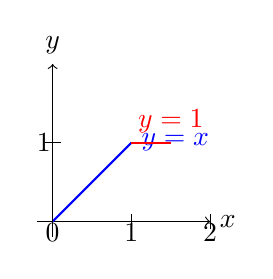
\begin{tikzpicture}
    % Axe x
    \draw[->] (-0.2,0) -- (2,0) node[right] {$x$};
    % Axe y
    \draw[->] (0,-0.2) -- (0,2) node[above] {$y$};
    
    % Graphe de y = x pour x dans [0, 1]
    \draw[thick, blue] (0,0) -- (1,1) node[right] {$y = x$};

    % Graphe de y = 1 pour x dans [1, 1.5]
    \draw[thick, red] (1,1) -- (1.5,1) node[above] {$y = 1$};

    % Marquage des points
    \foreach \x in {0, 1, 2} {
        \draw (\x, -0.1) -- (\x, 0.1) node[below] {$\x$};
    }
    \draw (-0.1, 1) -- (0.1, 1) node[left] {$1$};
\end{tikzpicture}
	\end{center}

 
\end{questions}
\begin{center}

\includegraphics[page=1,scale=0.87]{Tables_lois.pdf}
\end{center}

\begin{center}

\includegraphics[page=2,scale=0.87]{Tables_lois.pdf}
\end{center}

\begin{center}

\includegraphics[page=3,scale=0.87]{Tables_lois.pdf}
\end{center}
\begin{center}


\includegraphics[page=4,scale=0.87]{Tables_lois.pdf}
\end{center}
\begin{center}


\includegraphics[page=5,scale=0.87]{Tables_lois.pdf}
\end{center}
\begin{center}


\includegraphics[page=6,scale=0.87]{Tables_lois.pdf}
\end{center}



\end{document} 
